%%%%%%%%%%%%%%%%%%%%%%%%
% $Autor: MansourAhmadyPhoulady, RanjeetsingTawar, HemanthPrabhakaran$
% $Pfad: Car_Licence_Plate_Identification_with_a_JetsonNano$
% $Version: 4.0.0 $
%
% !TeX encoding = utf8
%
%%%%%%%%%%%%%%%%%%%%%%%%


\chapter{Conclusion}

In this project, we employ a systematic approach to interpret license plates (LP) from images, with the goal of generating plain text as output. The CLPD dataset encompasses a diverse range of images containing number plates, presenting various challenges such as illumination variations, weather conditions, and varying camera angles. These factors contribute to enhancing the model's resilience, enabling it to proficiently detect license plates even in challenging scenarios.

The project encompasses the integration of a software module that combines deep learning and image processing. The configuration of the input layer, hidden layer, dense layer, and output layer is fine-tuned to achieve optimal accuracy at a high processing speed. To prevent both underfitting and overfitting of the TensorFlow and Keras models, weight and bias adjustments are incorporated.

\section{Results}

The  project showcases a robust implementation of real-time car license plate detection using a Jetson Nano device. By leveraging Yolo,TensorFlow for object detection and EasyOCR for optical character recognition, the script efficiently identifies license plate regions in live video streams. Through careful filtering based on region size, the OCR process extracts accurate alphanumeric information from detected plates. The system not only visualizes the detection results with bounding boxes and labels but also records pertinent data, including the cropped license plate images and their corresponding text, facilitating further analysis. With error handling mechanisms in place, the script ensures smooth operation and offers a foundation for diverse applications such as vehicle tracking and parking management systems. Overall, this solution demonstrates the potential of deep learning and embedded hardware in enabling real-time license plate detection, highlighting its effectiveness in enhancing surveillance, security, and automation in various domains.

\begin{figure}
	\centering
	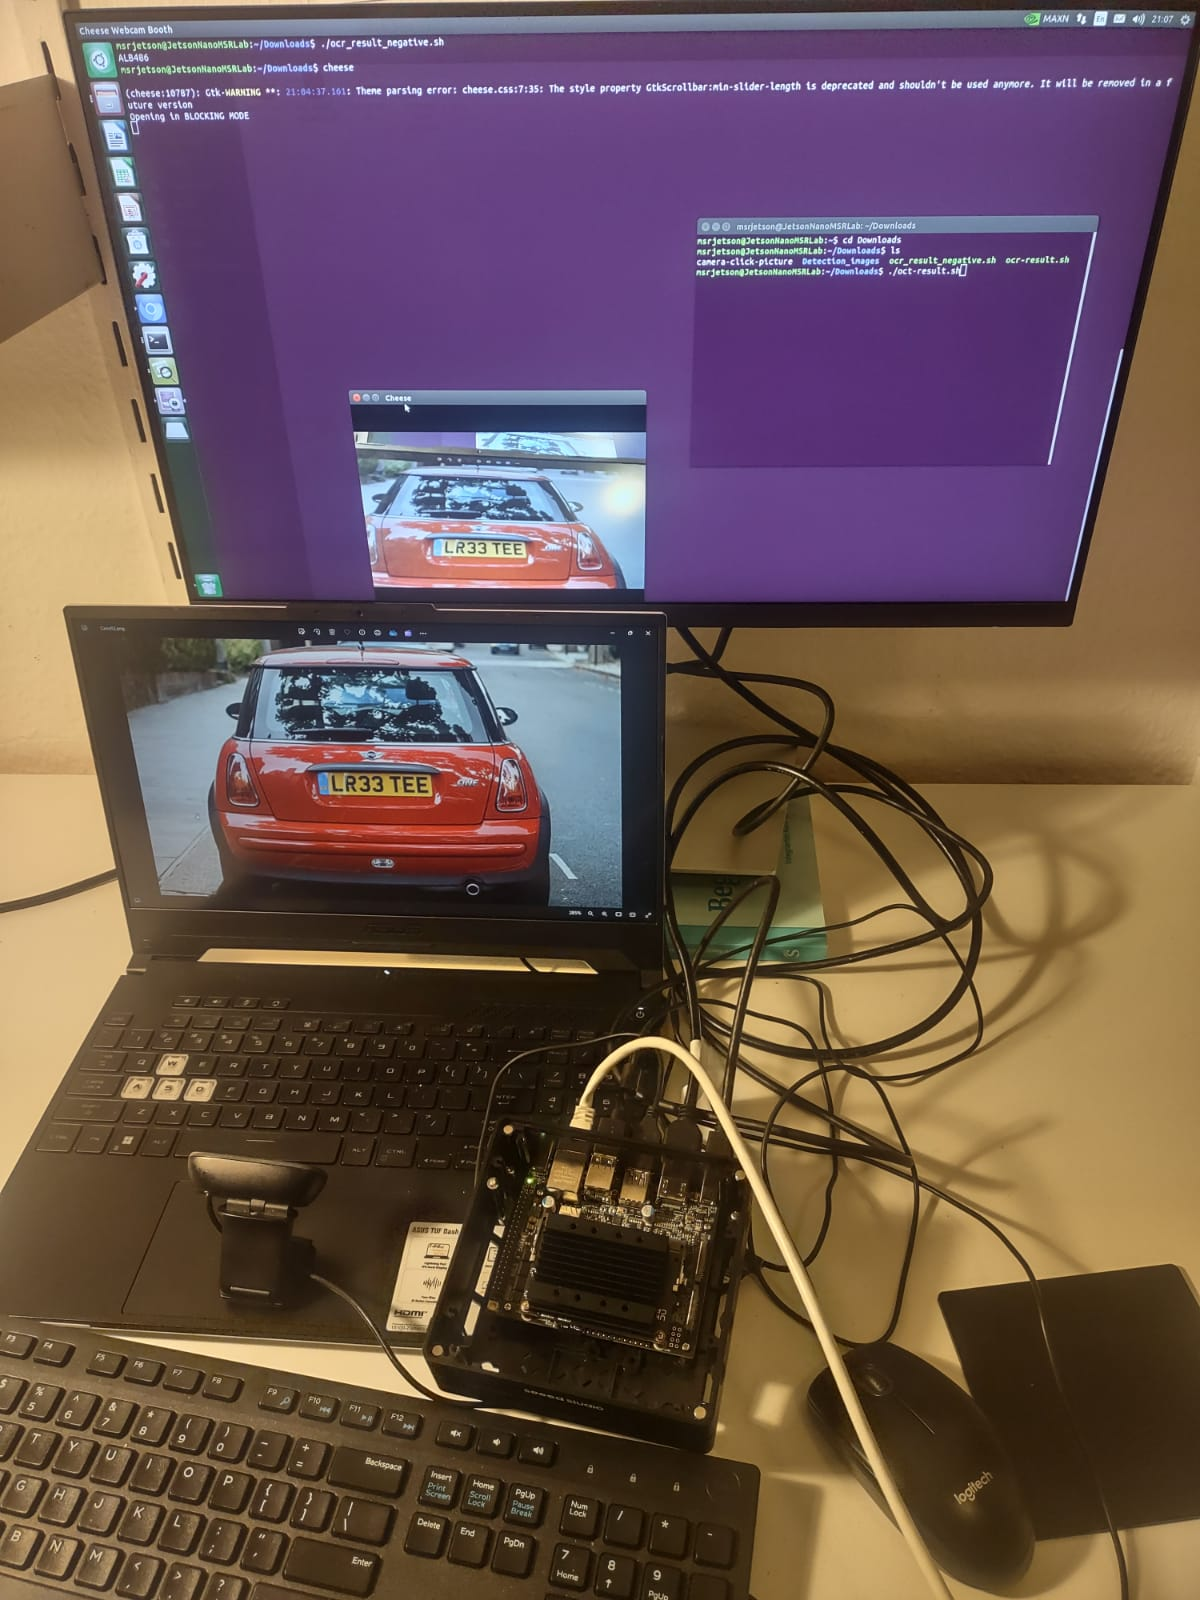
\includegraphics[width=0.7\linewidth]{Images/result}
	\caption{Result setup}
	\label{fig:result}
\end{figure}

	
\begin{figure}
	\centering
	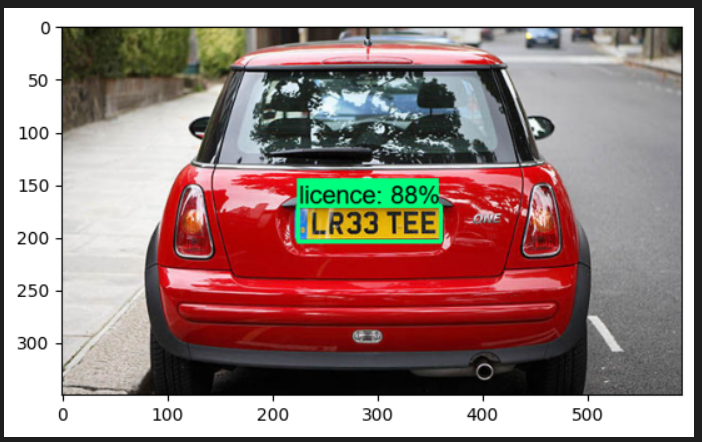
\includegraphics[width=0.7\linewidth]{Images/detection1}
	\caption{License Plate detection}
	\label{fig:License Plate detection}
\end{figure}

\begin{figure}
	\centering
	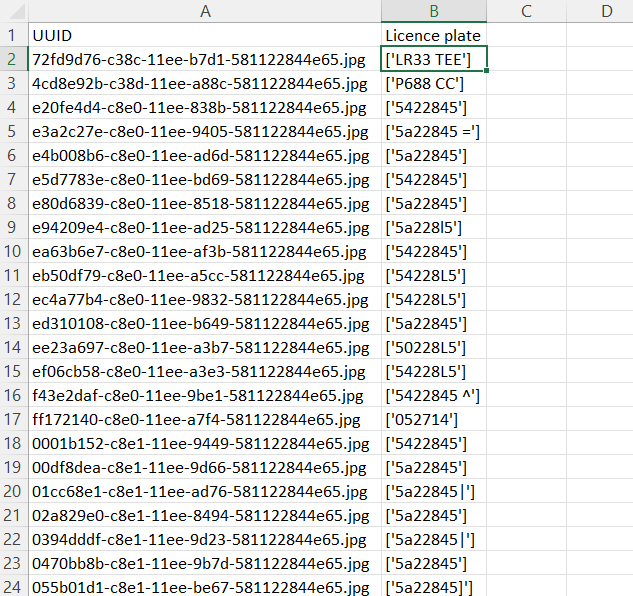
\includegraphics[width=0.7\linewidth]{Images/ResultCSV}
	\caption{Stored in CSV}
	\label{fig:Stored in CSV}
\end{figure}

\section{Improvements}
\subsection*{Introduction}
Challenges, solutions, and citations have been added to provide context and credibility to the project. Challenges may include limited computing power and hardware constraints, while solutions involve optimization techniques and leveraging Jetson Nano's capabilities. References are included to support the claims and solutions presented in the introduction.

\subsection*{Hardware}
A new camera module has been added to enhance data capture capabilities for license plate detection. Synchronization between hardware and software components has been achieved to ensure real-time processing of video streams. Conclusion emphasizes the importance of hardware optimization for efficient license plate detection on Jetson Nano. Hardware testing has been done along with parts and functions.

\subsection*{Software}
Required IDE data, system overview, installation steps, and conclusion have been added to the software section. The software setup includes the choice of IDE, programming languages, and libraries/frameworks used for license plate detection. Conclusion discusses the impact of software optimization on performance and accuracy.Previously licence plate was detected but text was not extracted but now detection, extraction, and storing is being done.

\subsection*{Technical Requirements}
Hardware and software bill of materials have been added with updated prices and links to documentation. Hardware bill of materials includes pictures and specifications of components used in the project.

\subsection*{KDD}
The structure of the KDD section has been aligned to cover data collection, preprocessing, model training, evaluation, and deployment. Examples of algorithms used for license plate detection, such as YOLO or SSD, have been included.

\subsection*{Conclusion}
To-do list and next steps have been added to the conclusion section, outlining future directions for the project. The conclusion summarizes achievements, challenges, and identifies areas for further improvement or research.

\subsection*{Data Sheets}
Data sheets for hardware components and software packages have been included to provide detailed information for readers.

\subsection*{Manual}
Welcome message, safety guidelines, maintenance instructions, troubleshooting steps, and images have been added to the manual section for user guidance and reference.

\subsection*{Camera Module}
Details of the new camera module, including specifications and integration with Jetson Nano, have been provided.

\subsection*{Packages}
Further reading resources, example versions of software packages used, and descriptions have been added to the packages section.

\subsection*{Flowchart}
Overall flow for the working of the project and explained each step involved in it. More description is added.

\subsection*{ML Pipeline}
The ML pipeline has been added from the scratch. Moreover, each and every step is explained properly in order to increase the understanding.

\section{Additions}


	
	In addition to the mentioned aspects of the project, here are some further considerations and components that could enhance its functionality and performance:
	
	\begin{enumerate}[label=\arabic*.]
		\item \textbf{Data Augmentation}: Implement techniques such as rotation, flipping, scaling, and adding noise to the images in the CLPD dataset. Data augmentation helps increase the diversity of training samples, which can improve the model's generalization ability and robustness to different environmental conditions.
		
		\item \textbf{Preprocessing Techniques}: Apply preprocessing techniques such as image resizing, normalization, and histogram equalization to standardize the input images before feeding them into the deep learning model. Preprocessing can help improve the model's accuracy by reducing the effects of variations in illumination and camera angles.
		
		\item \textbf{Model Architecture Selection}: Experiment with different deep learning architectures such as Convolutional Neural Networks (CNNs), Recurrent Neural Networks (RNNs), or a combination of both to find the most suitable architecture for license plate detection and interpretation. Consider architectures like YOLO (You Only Look Once) or SSD (Single Shot MultiBox Detector) for efficient real-time detection.
		
		\item \textbf{Hyperparameter Tuning}: Conduct a systematic search for optimal hyperparameters such as learning rate, batch size, and optimizer choice using techniques like grid search or random search. Hyperparameter tuning can significantly impact the performance of the deep learning model and improve its accuracy and convergence speed.
		
		\item \textbf{Transfer Learning}: Utilize pre-trained models such as VGG, ResNet, or MobileNet as feature extractors and fine-tune them on the CLPD dataset. Transfer learning can leverage the knowledge learned from large-scale datasets to improve the performance of the license plate detection and interpretation model, especially when the CLPD dataset is limited in size.
		
		\item \textbf{Ensemble Learning}: Combine predictions from multiple deep learning models or variations of the same model trained with different initializations or subsets of the training data. Ensemble learning can enhance the robustness and accuracy of the license plate interpretation system by leveraging diverse predictions from individual models.
		
		\item \textbf{Post-processing Techniques}: Apply post-processing techniques such as non-maximum suppression (NMS) to remove duplicate or overlapping bounding boxes generated by the deep learning model. Post-processing can help refine the final output and improve the accuracy of license plate localization and interpretation.
		
		\item \textbf{Deployment Considerations}: Design and implement a user-friendly interface for deploying the license plate interpretation system in real-world scenarios. Consider factors such as scalability, performance optimization, and compatibility with hardware platforms (e.g., Jetson Nano) for efficient deployment in edge computing environments or embedded systems.
	\end{enumerate}
	
\section{To Do}



\begin{enumerate}
	\item \textbf{Data Collection and Annotation}:
	\begin{itemize}
		\item Collect a diverse range of images containing number plates, considering variations in illumination, weather conditions, and camera angles.
		\item Annotate the images with bounding boxes around the license plates and corresponding text labels.
	\end{itemize}
	
	\item \textbf{Data Preprocessing}:
	\begin{itemize}
		\item Clean the dataset by removing noise and artifacts.
		\item Standardize the size and aspect ratio of images.
		\item Apply data augmentation techniques such as rotation, scaling, and flipping to increase the diversity of the dataset.
	\end{itemize}
	
	\item \textbf{Model Development}:
	\begin{itemize}
		\item Implement a deep learning model architecture for license plate detection and interpretation using TensorFlow and Keras.
		\item Configure the input layer, hidden layers, dense layers, and output layer based on the chosen architecture.
		\item Train the model on the preprocessed dataset, fine-tuning hyperparameters as needed.
	\end{itemize}
	
	\item \textbf{Evaluation}:
	\begin{itemize}
		\item Evaluate the trained model's performance using appropriate metrics such as precision, recall, and F1-score.
		\item Analyze the model's performance on challenging scenarios such as varying illumination and camera angles.
	\end{itemize}
	
	\item \textbf{Optimization}:
	\begin{itemize}
		\item Optimize the model for accuracy and processing speed by fine-tuning hyperparameters and adjusting the architecture.
		\item Implement techniques to prevent overfitting, such as dropout and regularization.
		\item Utilize GPU acceleration to speed up model training and inference.
	\end{itemize}
	
	\item \textbf{Integration and Deployment}:
	\begin{itemize}
		\item Integrate the trained model into a software module that combines deep learning and image processing techniques.
		\item Develop a user-friendly interface for uploading images and displaying the interpreted license plate text.
		\item Ensure compatibility with different operating systems and environments.
	\end{itemize}
	
	\item \textbf{Testing and Validation}:
	\begin{itemize}
		\item Test the integrated software module thoroughly on a variety of test images, including those with challenging conditions.
		\item Validate the accuracy and robustness of the license plate interpretation system across different scenarios.
	\end{itemize}
	
	\item \textbf{Documentation and Reporting}:
	\begin{itemize}
		\item Document the entire process, including data collection, model development, optimization, and deployment.
		\item Create user manuals and technical documentation for the software module.
		\item Prepare a comprehensive report detailing the project methodology, results, and future recommendations.
	\end{itemize}
\end{enumerate}


\section{Unanswered points}


	
	\begin{enumerate}
		\item \textbf{Localization Accuracy}:
		Explore techniques to improve the accuracy of license plate localization within images, especially in cases where license plates are partially obscured or distorted due to various factors such as reflections or occlusions.
		
		\item \textbf{Data Augmentation Strategies}:
		Investigate novel data augmentation strategies specifically tailored to address challenges present in the CLPD dataset, such as simulating realistic illumination variations, weather conditions, and camera angles to augment the training data effectively.
		
		\item \textbf{Model Generalization}:
		Evaluate the generalization capabilities of the trained model on unseen data sources or environments beyond the CLPD dataset, including different geographical regions with distinct license plate formats and characteristics.
		
		\item \textbf{Interpreting Special Characters}:
		Explore techniques to accurately interpret special characters or symbols commonly found in license plates, such as hyphens, spaces, and non-alphanumeric characters, which may vary across regions and countries.
		
		\item \textbf{Real-time Performance Optimization}:
		Investigate methods to optimize the model's inference speed and processing efficiency for real-time applications, potentially leveraging hardware acceleration or model compression techniques to achieve low-latency performance.
		
		\item \textbf{End-to-End System Integration}:
		Develop strategies for seamless integration of the license plate interpretation software module into existing systems or workflows, ensuring compatibility, scalability, and ease of deployment in diverse environments.
		
		\item \textbf{Robustness to Adversarial Attacks}:
		Assess the robustness of the model against adversarial attacks specifically crafted to deceive the license plate interpretation system, and explore techniques to enhance the model's resilience to such attacks.
		
		\item \textbf{User Interface Design}:
		Design and implement an intuitive user interface for the license plate interpretation software module, considering usability, accessibility, and user experience factors to facilitate smooth interaction and adoption by end-users.
		
		\item \textbf{Continuous Model Improvement}:
		Establish mechanisms for continuous model improvement and updating based on feedback from real-world usage, including techniques for monitoring model performance, collecting user feedback, and incorporating updates seamlessly.
		
		\item \textbf{Ethical and Legal Considerations}:
		Address ethical and legal considerations surrounding the use of license plate interpretation technology, including privacy implications, data protection measures, and adherence to relevant regulations and guidelines.
	\end{enumerate}
	
\section{Next Steps}



\subsection*{Data Preprocessing}
\begin{itemize}
	\item Clean and preprocess the CLPD dataset to remove noise, standardize image sizes, and enhance image quality.
	\item Employ techniques such as normalization, histogram equalization, and data augmentation to improve model performance.
\end{itemize}

\subsection*{Model Development}
\begin{itemize}
	\item Develop and train a deep learning model using TensorFlow and Keras for license plate detection and interpretation.
	\item Experiment with various architectures such as convolutional neural networks (CNNs), recurrent neural networks (RNNs), or a combination of both to achieve optimal accuracy.
\end{itemize}

\subsection*{Hyperparameter Tuning}
\begin{itemize}
	\item Fine-tune hyperparameters such as learning rate, batch size, and optimizer settings to optimize model performance.
	\item Utilize techniques like grid search or random search to efficiently search the hyperparameter space.
\end{itemize}

\subsection*{Evaluation Metrics}
\begin{itemize}
	\item Evaluate the trained model using appropriate performance metrics such as precision, recall, and F1-score to assess its accuracy and robustness.
	\item Utilize techniques like cross-validation or train-test split to ensure unbiased evaluation.
\end{itemize}

\subsection*{Deployment}
\begin{itemize}
	\item Deploy the trained model as a software module that integrates deep learning and image processing techniques.
	\item Develop a user-friendly interface for inputting images and displaying the interpreted license plate text.
\end{itemize}


\section{Future Work}

	
	
	\subsection*{Advanced Feature Extraction}
	\begin{itemize}
		\item Explore advanced feature extraction techniques such as edge detection, corner detection, and texture analysis to improve the model's ability to interpret license plates accurately, especially in challenging scenarios.
	\end{itemize}
	
	\subsection*{Multi-Language Support}
	\begin{itemize}
		\item Extend the model to support interpretation of license plates in multiple languages, considering the diversity of license plate formats and characters across different regions and countries.
	\end{itemize}
	
	\subsection*{Real-Time Processing}
	\begin{itemize}
		\item Optimize the model for real-time processing by implementing techniques such as model quantization, pruning, and optimization to reduce model size and inference latency.
	\end{itemize}
	
	\subsection*{Robustness to Environmental Conditions}
	\begin{itemize}
		\item Enhance the model's robustness to environmental conditions such as illumination variations, weather conditions, and varying camera angles by collecting additional annotated data and incorporating domain-specific augmentation techniques.
	\end{itemize}
	
	\subsection*{Integration with OCR Systems}
	\begin{itemize}
		\item Integrate the license plate interpretation module with optical character recognition (OCR) systems to further enhance accuracy and handle complex license plate designs and fonts.
	\end{itemize}
	
	By following these additional tasks and considering future work, you can further develop and improve the license plate interpretation project to achieve optimal accuracy and performance across various challenging scenarios.
	



